\documentclass[landscape]{article}
\usepackage[a4paper,margin=3mm,landscape]{geometry}
\usepackage[scaled=0.92]{helvet}
\usepackage{multicol, multirow}
\usepackage{makecell}
\usepackage{array} 
\usepackage[table]{xcolor}
\usepackage{enumitem} 
\usepackage{amssymb}
\usepackage{graphicx}
\setlist{nosep}

\graphicspath{{./images/}}

\pdfinfo{
    /Title (CS2106 Cheatsheet.pdf)
    /Creator (TeX)
    /Producer (pdfTeX 1.40.0)
    /Author (Selwyn Ang)
    /Subject (CS2106)
    /Keywords (CS2106, Cheatsheet, NUS, Introduction to Operating Systems) 
}

% Turn off header and footer
\pagestyle{empty}


\makeatletter
\DeclareRobustCommand\smaller{\@setfontsize\smaller{6pt}{6.5pt}}
\makeatother

% redefine section commands to use less space
\makeatletter
\renewcommand{\section}{\@startsection{section}{1}{0mm}%
  {-0.1ex plus -0.1ex minus -0.1ex}%
  {0.1ex plus .1ex minus 0.1ex}%
{\normalfont\small\bfseries}}
\renewcommand{\subsection}{\@startsection{subsection}{2}{0mm}%
  {-0.1ex plus -0.1ex minus -0.1ex}%
  {0.1ex plus .1ex minus 0.1ex}%
{\normalfont\scriptsize\bfseries}}
\renewcommand{\subsubsection}{\@startsection{subsubsection}{3}{0mm}%
  {-0.1ex plus -0.1ex minus -0.1ex}%
  {0.1ex plus .1ex minus 0.1ex}%
{\normalfont\smaller\bfseries}}%
\makeatother



\renewcommand{\familydefault}{\sfdefault}
\renewcommand\rmdefault{\sfdefault}
%  makes nested numbering (e.g. 1.1.1, 1.1.2, etc)
\renewcommand{\labelenumii}{\theenumii}
\renewcommand{\theenumii}{\theenumi.\arabic{enumii}.}
\renewcommand\labelitemii{•}
\renewcommand\labelitemiii{•}

\setlength{\parindent}{0pt}
\setlength{\parskip}{0pt plus 0.5ex}
\setlength{\columnsep}{0.2cm}
%% adjust spacing for all itemize/enumerate
\setlength{\leftmargini}{0.5cm}
\setlength{\leftmarginii}{0.5cm}
\setlist[itemize,1]{leftmargin=2mm,labelindent=1mm,labelsep=1mm}
\setlist[itemize,2]{leftmargin=2mm,labelindent=1mm,labelsep=1mm}
\setlist[itemize,3]{leftmargin=2mm,labelindent=1mm,labelsep=1mm}
\setlist[enumerate,1]{leftmargin=2mm,labelindent=1mm,labelsep=1mm}
\setlist[enumerate,2]{leftmargin=2mm,labelindent=1mm,labelsep=1mm}
\setlist[enumerate,3]{leftmargin=2mm,labelindent=1mm,labelsep=1mm}

% tightcenter
\newenvironment{tightcenter}{%
  \setlength\topsep{0pt}
  \setlength\parskip{0pt}
  \begin{center}
    }{%
  \end{center}
}

% boxed
\newenvironment{tightbox}{%
  \setlength\topsep{0pt}
  \setlength\parskip{0pt}
  \begin{center}
    \begin{tabular}{|@{\hspace{\dimexpr\fboxsep+0.5\arrayrulewidth}}c@{\hspace{\dimexpr\fboxsep+0.5\arrayrulewidth}}|}
      \hline
    }
    {%
    \\ \hline
    \end{tabular}
  \end{center}
}

% fixed width box
\newenvironment{fixedbox}[1][0.7]{
  \setlength\topsep{0pt}
  \setlength\parskip{0pt}
  \begin{center}
    \begin{tabular}{|>{\centering\arraybackslash}m{#1\linewidth}|}
    \hline
  }{
  \\ \hline
  \end{tabular}
  \end{center}
}

% definition of a new term
\usepackage{soul}
\definecolor{paleyellow}{RGB}{251,243,218}
\newcommand{\definition}[2][]{\sethlcolor{paleyellow}\hl{\textbf{#2}} #1  $\rightarrow$}
% inline definition
\newcommand{\ildefinition}[1]{\sethlcolor{paleyellow}\hl{\textbf{#1}}}

% important note (attention)
\newcommand{\attention}{{\color{red}\textbf{! }}}

% nice proof
\newenvironment{niceproof}[1][Proof]
{%
  \sbox0{\textit{#1}. }%
  \list{}{\labelwidth\wd0 \leftmargin\wd0 \labelsep 0pt }
\item[\usebox0]}
  {\endlist}


\usepackage{color, soul}
\usepackage{listings}
\usepackage{inconsolata}

\definecolor{codegreen}{rgb}{0,0.6,0}
\definecolor{codegray}{rgb}{0.5,0.5,0.5}
\definecolor{codepurple}{HTML}{C42043}
\definecolor{backcolour}{HTML}{F2F2F2}
\definecolor{bookColor}{cmyk}{0,0,0,0.90}

\newcommand{\code}[1]{\texttt{\sethlcolor{backcolour}\hl{$\,$#1$\,$}}}

% SQL code blocks
% define SQL styles
\lstdefinestyle{mySQL}{%
  language=SQL,
  backgroundcolor=\color{backcolour},
  commentstyle=\color{codegreen},
  keywordstyle=\color{codepurple},
  numberstyle=\numberstyle,
  stringstyle=\color{codepurple},
  basicstyle=\scriptsize\ttfamily,
  breaklines=true,
}



% --------------------------------------------------------

\begin{document}
\raggedright
\tiny
\begin{multicols*}{6}
    \setlength{\columnseprule}{0.25pt}

    \begin{tightcenter}
        \fbox{%
          \parbox{0.8\linewidth}{\centering \textcolor{black}{
              {\Large\textbf{CS2106 Finals}}
            \\ \normalsize{AY23/24 SEM 2}}
            \\ {\footnotesize \textcolor{gray}{github/SelwynAng}}
          }%
        }
    \end{tightcenter}
    
    \section{Synchronisation}
    \subsection{Race Conditions}
    \begin{itemize}
      \item Happens when execution of concurrent processes is non-deterministic
      \item Process which reaches the end first is the one that loses
      \item Each statement of a process consists of 
      \begin{enumerate}
        \item Load operation (Loads value from resource intro register)
        \item Register operation
        \item Store operation (Stores value from register into resource)
      \end{enumerate}
      \item Bad behavior occurs when different processes interleave
      \item \underline{No. of inter-leavings} = (nm!)/(m!)\textsuperscript{n} where there are \verb|n| threads, \verb|m| instructions per thread
      \item \underline{Relevant stages:} Load \& Store (eg. Thread A has 2 instructions, Thread B has 1 instruction $\rightarrow$ Thread A has 1L,1S,1L,1S, Thread B has 1L, 1S  $\rightarrow$ Insert B's L into 5 possible slots, insert B's S into 6 possible slots, but since only half of the permutations has L before S $\rightarrow$ No. of interleavings = 5*6/2 = 15)
    \end{itemize}
    
    \subsection{Critical Section}
    \begin{itemize}
      \item \textbf{Definition of Critical Section:} Section of code that performs a read, update \& write of a shared resource (code segment with race condition) $\rightarrow$ Only 1 process can execute in Critical Section at any point of time
      \item \textbf{Properties of Correct Critical Section Implementation}
      \begin{enumerate}
        \item \underline{Mutual Exclusion:} If a process is executing in CS, all other processes are prevented from entering CS
        \item \underline{Progress:} If no process in CS, 1 of waiting processes should be granted access
        \item \underline{Bounded Wait:} After a process P\textsubscript{i} requests to enter CS, there exists an upper-bound no. of times other processes can enter CS before P\textsubscript{i}
        \item \underline{Independence:} Process not executing in CS should never block other processes
      \end{enumerate}
      \item \textbf{Symptoms of Incorrect Synchronisation}
      \begin{enumerate}
        \item \underline{Deadlock:} All processes are blocked $\rightarrow$ No Progress
        \item \underline{Livelock:} Processes keep changing state to avoid deadlock (processes are not considered blocked) $\rightarrow$ No Progress
        \item \underline{Starvation:} Some processes are blocked forever
      \end{enumerate}
    \end{itemize}

    \subsection{Assembly-level Implementation of CS}
    \begin{itemize}
      \item Mechanism provided by processor
    \end{itemize}
    \subsubsection{Test \& Set}
    \begin{itemize}
      \item \textbf{Overview:} Takes a memory address M $\rightarrow$ Returns current content at M \& Sets content of M to 1
      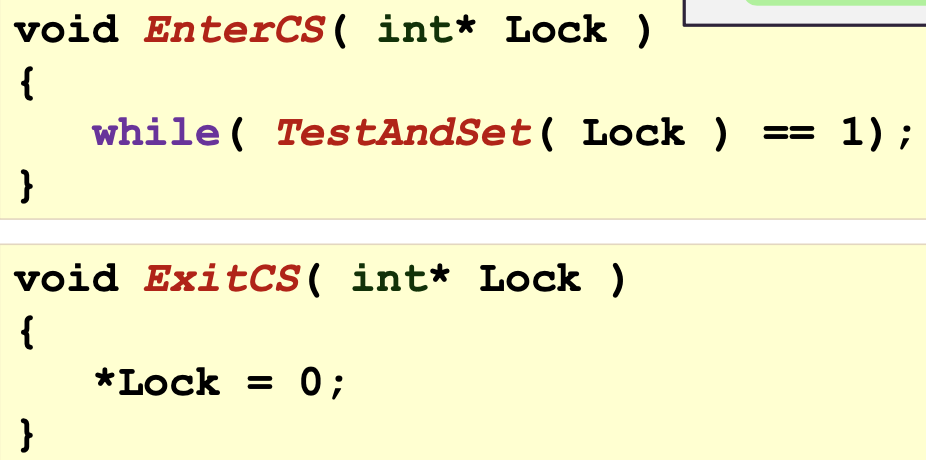
\includegraphics[width=0.75\linewidth]{1_testandset.png}
      \item \textbf{Procedure:}
      \begin{enumerate}
        \item Initially, Lock == 0 $\rightarrow$ \verb|TestAndSet(Lock)| returns 0 and sets Lock == 1
        \item While loop of 1st process exits $\rightarrow$ 1st process entered CS successfully
        \item Other processes cannot enter CS as Lock == 1 $\rightarrow$ While loops will not exit for those processes
        \item Upon exiting CS, set Lock == 0 $\rightarrow$ Other processes can enter CS
      \end{enumerate}
      \item \textbf{Cons:} Employs busy waiting for blocked processes (keeps checking while loop condition until it is safe to enter CS) $\rightarrow$ Waste of processing power
    \end{itemize}

    \subsection{High-level Language Implementation of CS}
    \begin{itemize}
      \item Utilize only normal programming constructs
      \item \textbf{Flaws of certain implementations:}
      \begin{enumerate}
        \item \underline{Preemption:} P\textsubscript{0} gets preempted after while loop $\rightarrow$ P\textsubscript{1} sees that lock == 0, exits while loop \& sets lock == 1 $\rightarrow$ P\textsubscript{1} hands control back to P\textsubscript{0} while lock == 1 \& P\textsubscript{1} is in CS $\rightarrow$ P\textsubscript{0} has checked the while loop before already \& would just enter CS (Mutual Exclusion violated)
        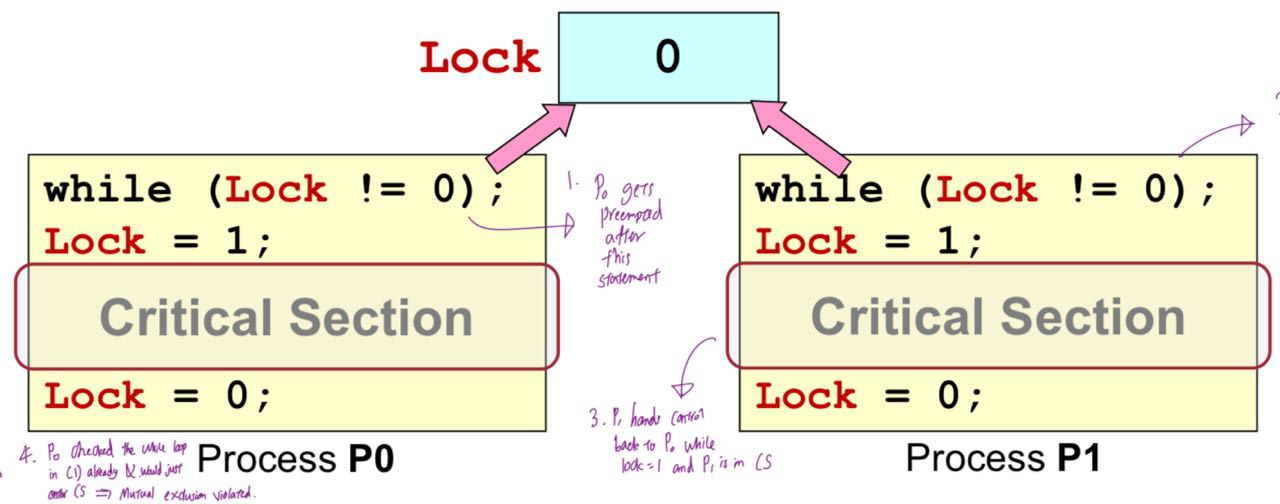
\includegraphics[width=0.9\linewidth]{2_attempt1.jpg}
        \item \underline{Disabling \& enabling interrupts:} Prevents context switch when a process is in CS (preemption requires interrupts), but \\ (1): Process crashes in CS, no way to re-enable interrupts $\rightarrow$ system shuts down; (2): Busy waiting employed; (3): Permission needed to disable/enable interrupts; (4): Ineffective on multi-CPU systems (If processes on different CPUs, disabling a process' interrupts will only disable interrupts on its CPU, other CPU not affected)
        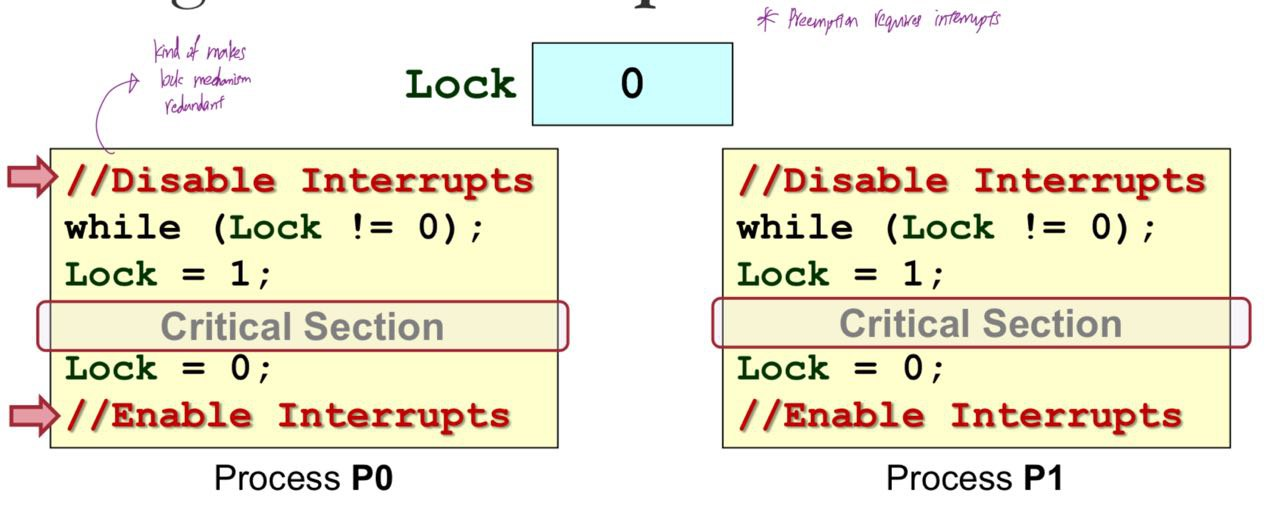
\includegraphics[width=0.9\linewidth]{3_attempt2.jpg}
        \item \underline{Failure to enter CS:} P\textsubscript{0} does not manage to enter CS, P\textsubscript{1} can starve $\rightarrow$ fufils Mutual Exclusion, but violates Independence
        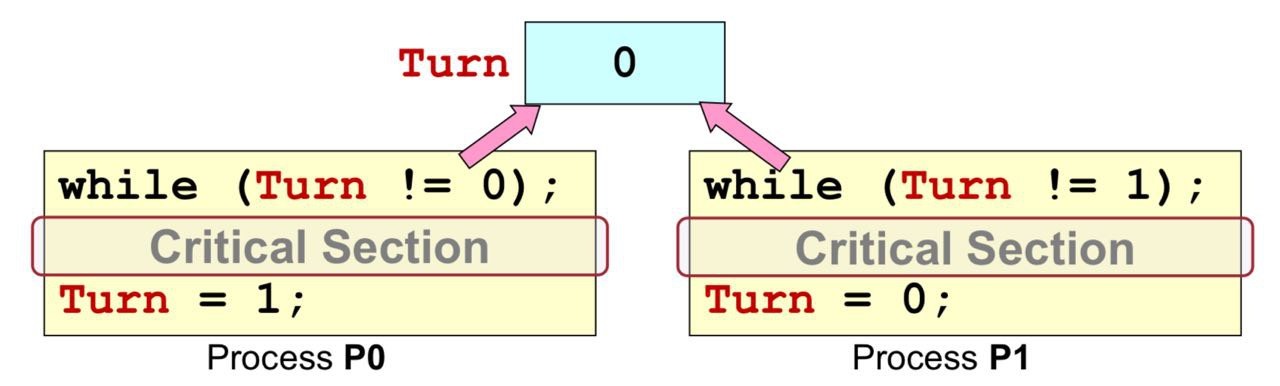
\includegraphics[width=0.9\linewidth]{4_attempt3.jpg}
        \item \underline{Deadlock:} P\textsubscript{0} sets \verb|Want[0] == 1| \& preempted $\rightarrow$ P\textsubscript{1} sets \verb|Want[1] == 1| $\rightarrow$ Both processes are stuck at while loop
        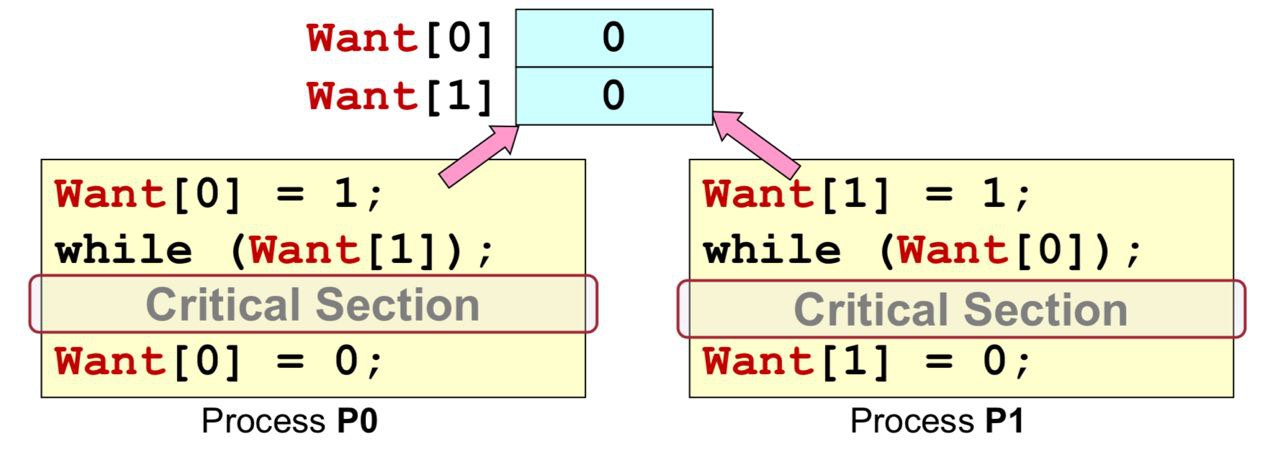
\includegraphics[width=0.9\linewidth]{5_attempt4.jpg}
      \end{enumerate}
    \end{itemize}
    \subsubsection{Peterson Algorithm}
    \begin{itemize}
      \item \textbf{Overview (Analogy of boarding bus where bus is CS):} A process will WANT to enter CS \& then gives TURN to other process $\rightarrow$ If P\textsubscript{i} gives TURN to P\textsubscript{j} but P\textsubscript{j} don't want to enter CS, P\textsubscript{i} will enter CS $\rightarrow$ Final TURN value ultimately determines which process can enter CS (only when both processes WANT to enter CS)
      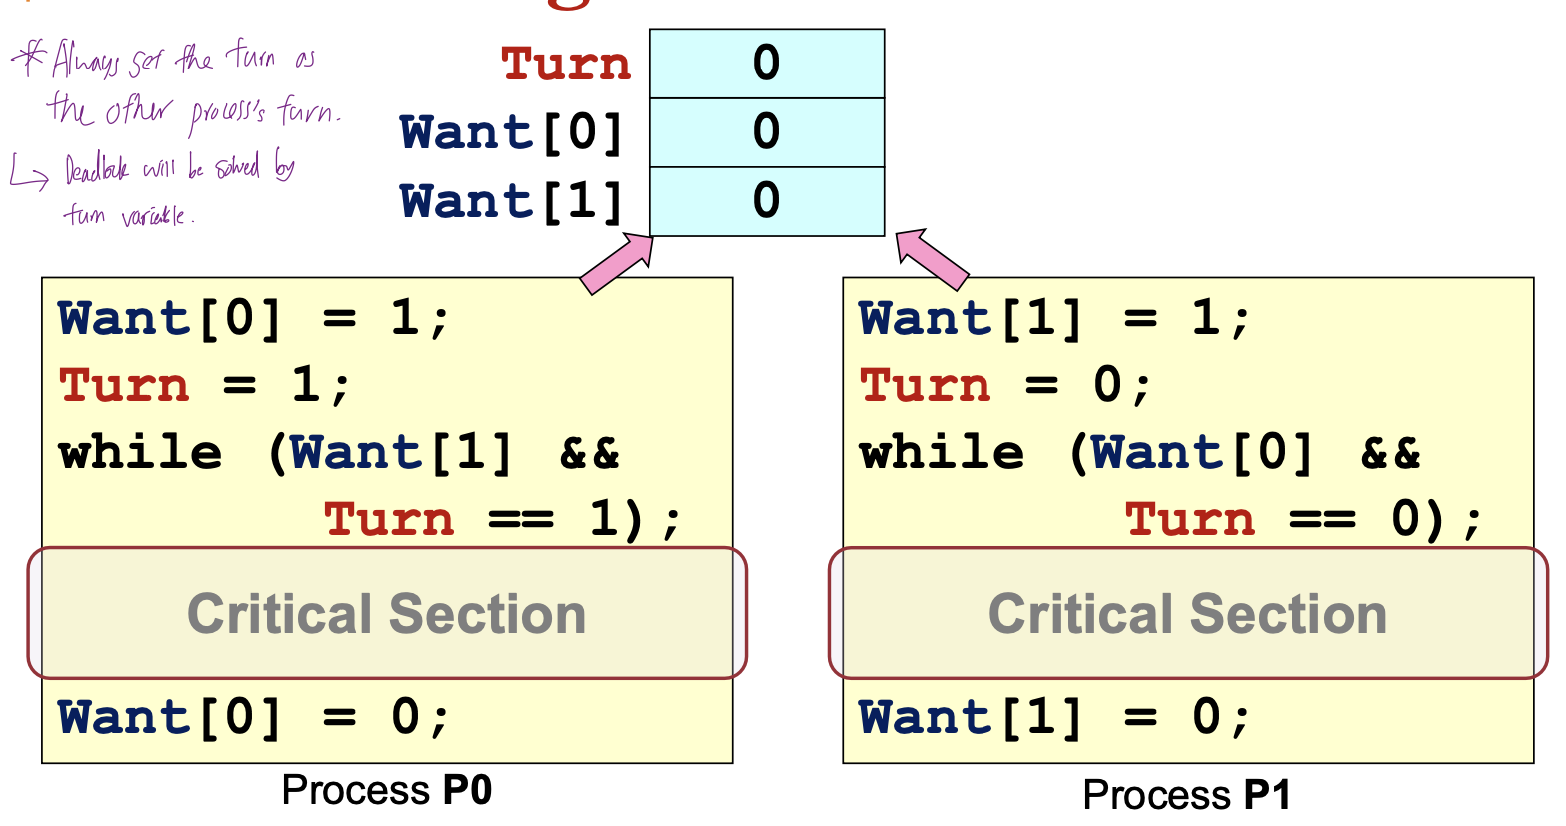
\includegraphics[width=0.9\linewidth]{6_peterson.png}
      \item \textbf{Scenarios:}
      \begin{enumerate}
        \item Both P\textsubscript{0} \& P\textsubscript{1} WANT, TURN == 0 $\rightarrow$ P\textsubscript{0} enters CS, P\textsubscript{1} blocked
        \item Both P\textsubscript{0} \& P\textsubscript{1} WANT, TURN == 1 $\rightarrow$ P\textsubscript{0} blocked, P\textsubscript{1} enters CS
        \item P\textsubscript{0} WANT \& P\textsubscript{1} don't WANT, TURN == 1 $\rightarrow$ P\textsubscript{0} enters CS, P\textsubscript{1} will get blocked even if it WANTS \& sets TURN == 0 eventually
        \item P\textsubscript{0} don't WANT \& P\textsubscript{1} WANT, TURN == 0 $\rightarrow$ P\textsubscript{1} enters CS, P\textsubscript{0} will get blocked even if it WANTS \& sets TURN == 1 eventually
      \end{enumerate}
    \end{itemize}

    \subsection{Semaphores Implementation of CS}
    \subsubsection{Semaphores}
    \begin{itemize}
      \item Provides a way to block a number of processes \& a way to unblock $\geq$ 1 sleeping process
      \item A semaphore \verb|S| contains an integer value (Initialised to any non-negative value)
      \item Given S\textsubscript{initial} $\geq$ 0, S\textsubscript{current} = S\textsubscript{initial} + No. of signal operations executed - No. of wait operations completed
      \item \textbf{Semaphore Operations:}
      \begin{enumerate}
        \item \verb|Wait(S)|: If \verb|S| $\leq$ 0, process blocks $\rightarrow$ After process unblocks, decrement \verb|S| (Code: \verb|P(Semaphore S) { while(S <= 0); S --;}|)
        \item \verb|Signal(S)|: Increment \verb|S| \& unblocks 1 blocked process if any (Signal never blocks) (Code: \verb|V(Semaphore S) {S++;}|)
      \end{enumerate}
      \item \textbf{Semaphore Types:}
      \begin{enumerate}
        \item \underline{General Semaphore:} S $\geq$ 0
        \item \underline{Binary Semaphore:} S = 0 or 1 (General semaphores can be mimicked by binary semaphores)
      \end{enumerate}
      \item \textbf{Semaphores in Critical Section:}
      \begin{itemize}
        \item Place \verb|Wait(S)| before CS \& \verb|Signal(S)| after CS $\rightarrow$ ensures mutual exclusion
        \item \underline{Binary Semaphore Implementation:}(1): S\textsubscript{initial} = 1 \& there are 2 processes P\textsubscript{0} \& P\textsubscript{1} trying to access shared resource in CS; (2): P\textsubscript{0} calls \verb|Wait(S)| $\rightarrow$ Since S = 1, it does not block \& proceeds to decrement S to 0 $\rightarrow$ P\textsubscript{0} enters CS; (3):  P\textsubscript{1} calls \verb|Wait(S)| $\rightarrow$ Since S = 0,  P\textsubscript{1} blocks \& cannot enter CS; (4):  P\textsubscript{0} finishes CS \& calls \verb|Signal(S)| $\rightarrow$ S incremented back to 1; (5):  P\textsubscript{1} becomes unblocked, S decremented back to 0, P\textsubscript{1} enters CS, calls \verb|Signal(S)| \& increments S to 1
        \item \underline{General Semaphore Implementation:} Can be generalised from binary semaphore implementation (eg. S\textsubscript{initial} = 2, 3 processes trying to access 2 shared resources in CS)
      \end{itemize}
    \end{itemize}
    \subsubsection{Proofs of Semaphore Correctness}
    \begin{enumerate}
      \item \textbf{Semaphore ensuring mutex in CS:} N\textsubscript{CS} = No. of processes in CS = \#Wait(S) - \#Signal(S) $\rightarrow$ Given S\textsubscript{initial} = 1, S\textsubscript{current} = 1 + \#Signal(S) - \#Wait(S) $\rightarrow$ S\textsubscript{current} + N\textsubscript{CS} = 1 $\rightarrow$ Since S\textsubscript{current} $\geq$ 0, hence N\textsubscript{CS} $\leq$ 1
      \item \textbf{Semaphore preventing deadlock:} Deadlock means all processes stuck at \verb|Wait(S)| $\rightarrow$ S\textsubscript{current} = 0 \& N\textsubscript{CS} = 0 $\rightarrow$ But S\textsubscript{current} + N\textsubscript{CS} = 1 (Contradiction)
      \item \textbf{Semaphore preventing starvation:} Suppose P\textsubscript{1} is blocked at \verb|Wait(S)|, P\textsubscript{2} is in CS $\rightarrow$ P\textsubscript{2} exits CS with \verb|Signal(S)| $\rightarrow$ If no other processes sleeping, P\textsubscript{1} wakes up OR If there are other processes, P\textsubscript{1} eventually wakes up (assuming fair scheduling)
    \end{enumerate}
    \subsubsection{Disadvantages of Semaphores}
    \begin{itemize}
      \item Can result in Deadlock if used incorrectly
      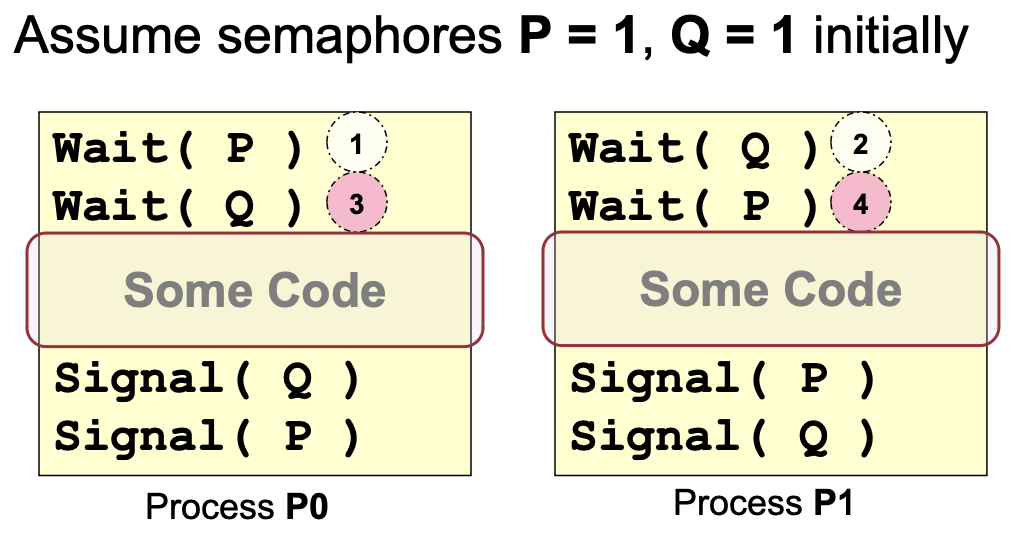
\includegraphics[width=0.75\linewidth]{7_semaphore_deadlock.png}
      \begin{enumerate}
        \item P\textsubscript{0} calls \verb|Wait(P)| \&  P\textsubscript{1} calls \verb|Wait(Q)| $\rightarrow$ P = 0 \& P = 0
        \item P\textsubscript{0} calls \verb|Wait(Q)| \&  P\textsubscript{1} calls \verb|Wait(P)| $\rightarrow$ P\textsubscript{0} \& P\textsubscript{1} both become blocked as P = 0 \& Q = 0 already
        \item P is held by P\textsubscript{0} \& Q is held by P\textsubscript{1} $\rightarrow$ Signal of both processes cannot be reached to increment the semaphores (both processes reach deadlock)
      \end{enumerate}
    \end{itemize}
    
    \subsection{Classical Synchronisation Problems}
    \subsubsection{Producer-Consumer Problem}
    \begin{itemize}
      \item \textbf{Overview:}
      \begin{itemize}
        \item Processes share a bounded buffer of size K
        \item \underline{Constraints:} (1): Producers produce items to insert into buffer only when buffer is not full; (2): Consumers remove items from buffer only when buffer is not empty; (3): Producer should not produce when another producer is producing; (4): Consumer should not remove when another consumer is removing; (5): Producer \& consumer should not produce \& consume at same time
      \end{itemize}
      \item \textbf{Naive Solution (Busy waiting):}
      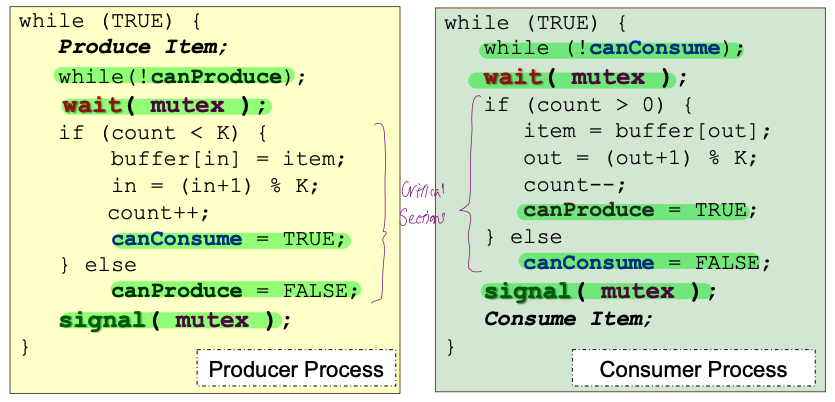
\includegraphics[width=1.0\linewidth]{8_reader_writer_naive.png}
      \begin{itemize}
        \item Initially, \verb|canProduce|=TRUE, \verb|canConsume|=FALSE, \verb|mutex|=1
        \item Correctly solves problem, but busy waiting is still used in while loop
      \end{itemize}
      \item \textbf{3 Semaphores Solution (Blocking version):}
      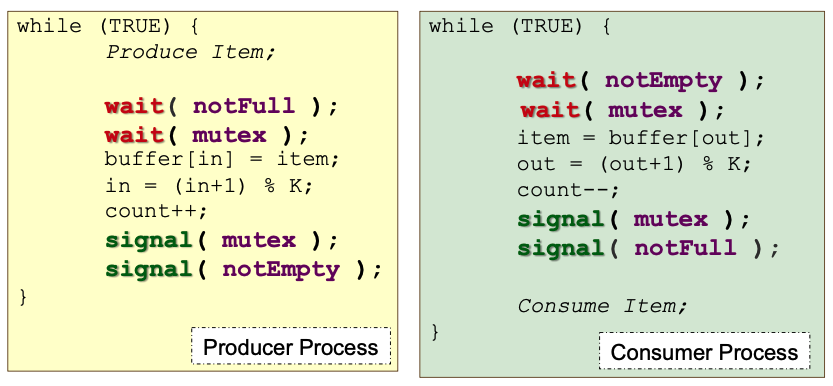
\includegraphics[width=1.0\linewidth]{9_three_sema_slon.png}
      \begin{itemize}
        \item \verb|mutex|: binary semaphore that is used to acquire \& release the lock (ensures only 1 producer/consumer in CS); \verb|notFull|: general semaphore whose initial value == K (represents no. of empty slots); \verb|notEmpty|: general semaphore whose initial value == 0 (represents no. of occupied slots)
        \item \underline{Producer perspective:} Producer calling \verb|Wait(notFull)| sees notFull \textgreater 0, indicating buffer still has space $\rightarrow$ calls \verb|Wait(mutex)| to acquire lock, inserts item, calls \verb|Signal(mutex)| to release lock $\rightarrow$ Producer calls \verb|Signal(notEmpty)| to $\uparrow$ value of \verb|notEmpty|, indicating 1 item inserted (If \verb|notFull| == 0, buffer is full \& producer is blocked until a consumer removes an item \& calls \verb|Signal(notFull)|)
        \item \underline{Consumer perspective:} Consumer calling \verb|Wait(notEmpty)| sees notEmpty \textgreater 0, indicating buffer still has items $\rightarrow$ calls \verb|Wait(mutex)| to acquire lock, removes item, calls \verb|Signal(mutex)| to release lock $\rightarrow$ Consumer calls \verb|Signal(notFull)| to $\uparrow$ value of \verb|notFull|, indicating 1 item removed (if \verb|notEmpty| == 0, buffer is empty \& consumer is blocked until a producer inserts an item \& calls \verb|Signal(notEmpty)|)
      \end{itemize}
    \end{itemize}

    \subsubsection{Reader-Writer Problem}
    \begin{itemize}
      \item \textbf{Overview:}
      \begin{itemize}
        \item Processes share a data structure where a Reader retrieves information \& a Writer modifies information
        \item \underline{Constraints:} (1): Only 1 writer can access data structure (no other writer or reader should access at same time); (2): Reader can access data structure at same time as other Readers \\
      \end{itemize}
      \item \textbf{Semaphore Solution:} \\
      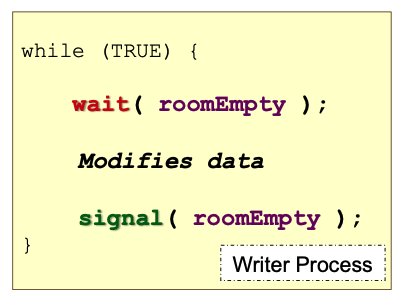
\includegraphics[width=0.45\linewidth]{10_writer.png}
      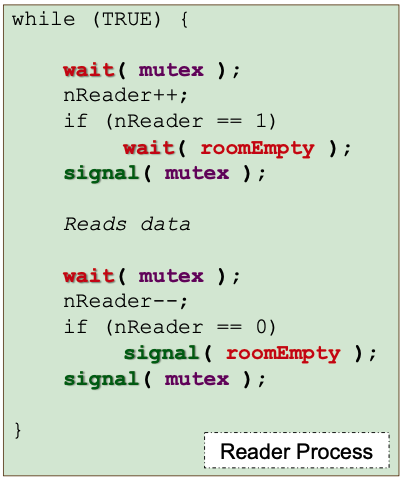
\includegraphics[width=0.5\linewidth]{11_reader.png}
      \begin{itemize}
        \item \verb|nReader|: Integer variable initialised to 0 (keeps track of current no. of readers), \verb|roomEmpty|: initialised to 1 (keeps track of presence of readers \& writers currently accessing data structure), \verb|mutex|: initialised to 1, ensure mutual exclusion when \verb|nReader| is updated (shared variable which can be updated by multiple readers)
        \item \underline{Writer perspective:} Writer calls \verb|Wait(roomEmpty)|, indicating that no other reader/writer can access data structure $\rightarrow$ Enters CS, modifies data $\rightarrow$ calls \verb|Signal(roomEmpty)|, other readers/writers can now access
        \item \underline{Reader perspective:} Reader tries to access data structure \& increments \verb|nReader| $\rightarrow$ If \verb|nReader| == 1, it means there is $\geq$ 1 reader present $\rightarrow$ Reader calls \verb|Wait(roomEmpty| which prevents writer from accessing data structure $\rightarrow$ After reader is done, \verb|nReader| is decremented $\rightarrow$ If \verb|nReader| == 0, there are no more readers present, can call \verb|Signal(roomEmpty)|, allowing writer access
        \item Reader is not bounded roomEmpty semaphores as multiple readers can access data structure at same time
        \item \underline{Potential issue:} If reader arrival rate \textgreater reader depart rate $\rightarrow$ \verb|nReader| may not be able to decrement to 0 \& just keeps increasing $\rightarrow$ writers will forever be blocked since \verb|Signal(roomEmpty)| will not be called
      \end{itemize}
    \end{itemize}

    \subsubsection{Dining Philosopher Problem}
    \begin{itemize}
      \item \textbf{Overview:} 5 philosophers are seated around a table, 5 single chopstick placed between each pair of philosophers $\rightarrow$ When any philosopher wants to eat, he has to acquire both left \& right chopsticks (Have to devise deadlock-free \& starve-free way for philosopher to eat)
      \item \textbf{Naive method:} \verb|Think(); takeChpStk(LEFT); takeChpStk(RIGHT);| \verb|Eat(); putChpStk(LEFT); putChpStk(RIGHT);| \\ All pick up left chpstk together $\rightarrow$ each philosopher cannot pick up right chpstk(Deadlock occurs \& cannot eat); Can make philosopher put down left chpstk if right chpstk cannot be acquired $\rightarrow$ Left chpstk will be taken up \& down repeatedly (livelock occurs)
      \item \textbf{Naive method with Mutex:} Surround above code with \verb|Wait(mutex)| \& \verb|Signal(mutex)| $\rightarrow$ but only 1 philosopher can take, eat, put at a time (inefficient)
      \item \textbf{Tanenbaum Solution:} \\
      \begin{multicols}{2}
        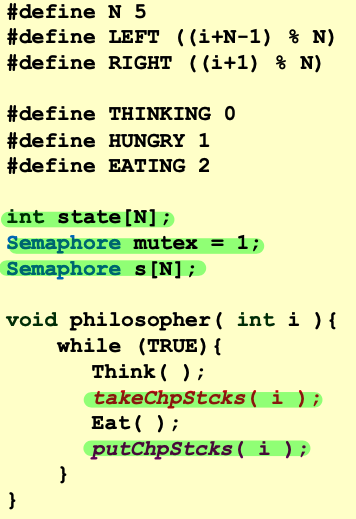
\includegraphics[width=1.0\linewidth]{12_tanenbaum.png} \\
        \columnbreak
        void takeChpStcks(i) \{ wait(mutex); state[i] = HUNGRY; safeToEat(i); signal(mutex); wait(s[i]);\} \hrule
        void safeToEat(i) \{ if (state[i] == HUNGRY \&\& state[LEFT] != EATING \&\& state[RIGHT] != EATING) \{ state[i] = EATING; signal(s[i]); \} \} \hrule
        void putChpStcks(i) \{ wait(mutex); state[i] = THINKING; safeToEat(LEFT); safeToEat(RIGHT); signal(mutex); \}
        \end{multicols}
        \begin{itemize}
          \item \verb|mutex|: binary semaphore that ensures only 1 philosopher can carry out 1 action; \verb|s[N]|: array of binary semaphores with 1 semaphore per chpstck
          \item \underline{Philosopher perspective:} Become hungry \& checks if it is safe to eat (if he is hungry \& his neighbors are both not hungry $\rightarrow$ calls signal on his own chpstck to show that he can acquire his chpstck as it is not used by his neighbors) $\rightarrow$ Calls wait on his own chpstck so he can acquire his own chpstck if it is not taken by his neighbor OR become blocked if his own chpstck is taken by his neighbor $\rightarrow$ proceeds to eat \& puts down chpstick, change state to thinking \& checks if it is safe to eat for his neighbors
        \end{itemize}
      \item \textbf{Limited Eater Solution:} Just leave 1 empty seat (no deadlock can happen when 4 philosophers share 5 single chpstks as 1 philosopher can access 2 chpstks at 1 time)
    \end{itemize}

    \subsection{POSIX Semaphores}
    \begin{itemize}
      \item \textbf{Mutex:} \verb|pthread_mutex| (Lock: \verb|pthread_mutex_lock()|, Unlock: \verb|pthread_mutex_unlock()|)
      \item \textbf{Conditional Variables:} \verb|pthread_cond| (Wait: \verb|pthread_cond_wait()|, Signal: \verb|pthread_cond_signal()|, Broadcast: \verb|pthread_cond_broadcast|)
    \end{itemize}

    \section{Memory (Contiguous)}
    \subsection{Basics of Memory}
    \begin{itemize}
      \item \textbf{Memory Hardware}: Physical memory (RAM) can be treated as an array of bytes (each byte has unique physical address)
      \item \textbf{Memory Usage of Process:} Consists of Text (instructions), Data (global variables), Heap (dynamic allocation), Stack (function invocation)
      \item \textbf{Memory Management by OS:} OS allocates memory space to new processes, manage memory space for processes, protect memory space of processes from each other, provides memory-related system calls to processes, manage memory space for internal use
    \end{itemize}
    
    \subsection{Memory Abstraction}
    \begin{itemize}
      \item \textbf{Without Memory Abstraction:} Process directly uses physical address (No mapping needed, but 2 processes can occupy same physical memory if both processes assume memory starts at 0 $\rightarrow$ hard to protect memory space)
      \item \textbf{Without Memory Abstraction (Address Relocation):} Recalculate memory references when process is loaded into memory by adding unique offset to all memory references in a process (but slow loading time, not easy to distinguish memory reference from normal integer constant)
      \item \textbf{Without Memory Abstraction (Base \& Limit Registers):}
      \begin{itemize}
        \item \underline{Base Register:} Initialised to starting address of process memory space at loading time (All memory references are compiled as offset from base register)
        \item \underline{Limit Register:} Indicates range of memory space of current process
        \item \underline{Cons:} Every access: 1 addition (\verb|Actual = Base + Addr|) \& 1 comparison (\verb|Actual < Limit|)
      \end{itemize}
      \item \textbf{Logical Address:} How process views its memory space (Logical address != Physical address, mapping required)
    \end{itemize}

    \subsection{Contiguous Memory Management}
    \begin{itemize}
      \item \textbf{Assumptions:} (1): Each process occupies a contiguous memory region, (2): Physical memory is large enough to contain $\geq$ 1 processes with complete memory space
      \item \textbf{Memory Partition:} Contiguous memory region allocated to a single process (eg. RAM has 4 partition $\rightarrow$ RAM can store 4 processes) ~ 2 allocation schemes (Fixed size \& Variable)
    \end{itemize}

    \subsection{Fixed-size Partitioning}
    \begin{itemize}
      \item OS maintains information about free \& occupied partition via an ARRAY
      \item Memory is split into equal, fixed-size partitions (1 process occupies 1 partition)
      \item \underline{Pros:} Easy to manage, fast to allocate (every free partition is same size, no need to choose)
      \item \underline{Cons:} Partition size needs to be large enough to contain the largest process (Smaller process will waste space $\rightarrow$ Internal Fragmentation)
      \item \textbf{Internal Fragmentation:} Process fails to occupy whole partition, left over space WITHIN partition is wasted
    \end{itemize}

    \subsection{Dynamic Partitioning}
    \begin{itemize}
      \item OS maintains information about free \& occupied partition via a LINKED LIST (list of partitions \& holes with size values)
      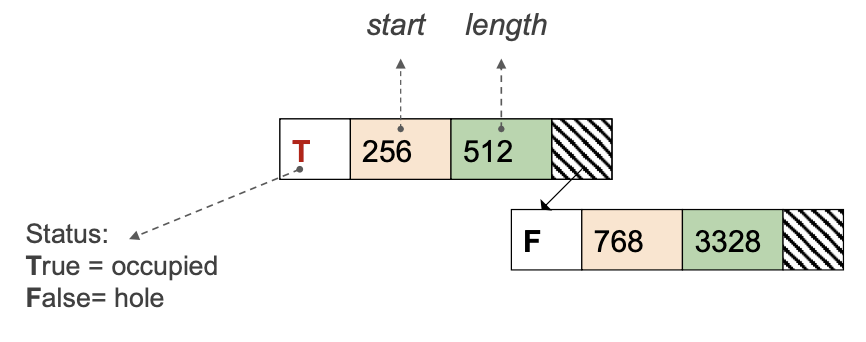
\includegraphics[width = 0.8\linewidth]{13_dynamic_partitioning_list.png}
      \item Partition is created based on actual size of process
      \item \underline{Pros:} Flexible, removes Internal Fragmentation issue
      \item \underline{Cons:} Need to maintain more info in OS (linked list), takes more time to locate appropriate region, results in External Fragmentation
      \item \textbf{External Fragmentation:} Free memory space is created upon process creation/termination/swapping (wasted), but can be mitigated by merging holes by moving occupied partitions to create larger hole (can fit process)
      \item \textbf{Allocation Algorithms:} OS maintains a list of partitions \& holes $\rightarrow$ Need to locate partition of size N (size of process == N) $\rightarrow$ Search for hole with size M \textgreater N $\rightarrow$ Split hole into N \& M-N (N is new partition, M-N is new hole)
      \begin{enumerate}
        \item \underline{First-fit:} Take 1st hole that is large enough (Fastest runtime since search stops once 1st hole found, but least efficient for memory usage as keeps assigning at beginning of list $\rightarrow$ many holes at end of memory)
        \item \underline{Next-fit:} Similar to First-fit, but search from last allocated block \& wrap around circular linked list (ensures memory at the end is utilized too)
        \item \underline{Best-fit:} Find smallest hole that is large enough (but slow runtime because need to search whole list for smallest hole)
        \item \underline{Worst-fit:} Find largest hole (slow runtime because need to search whole list for largest hole, but more efficient memory-wise as less small holes formed after assigning a process $\rightarrow$ can fit more processes in the future)
      \end{enumerate}
      \item \textbf{Buddy System Allocation:}
      \begin{itemize}
        \item \underline{Overview:} Free block is split into half repeatedly to meet request size (2 halves form buddy blocks), buddy blocks merge to form larger block when they are both free
        \item \underline{Implementation Structure:} An array \verb|A[0...K]| is maintained where 2\textsuperscript{K} is largest block size that can be allocated, each \verb|A[J]| is a linked list keeping track of free blocks of size 2\textsuperscript{J}, Each free block is indicated by starting address
        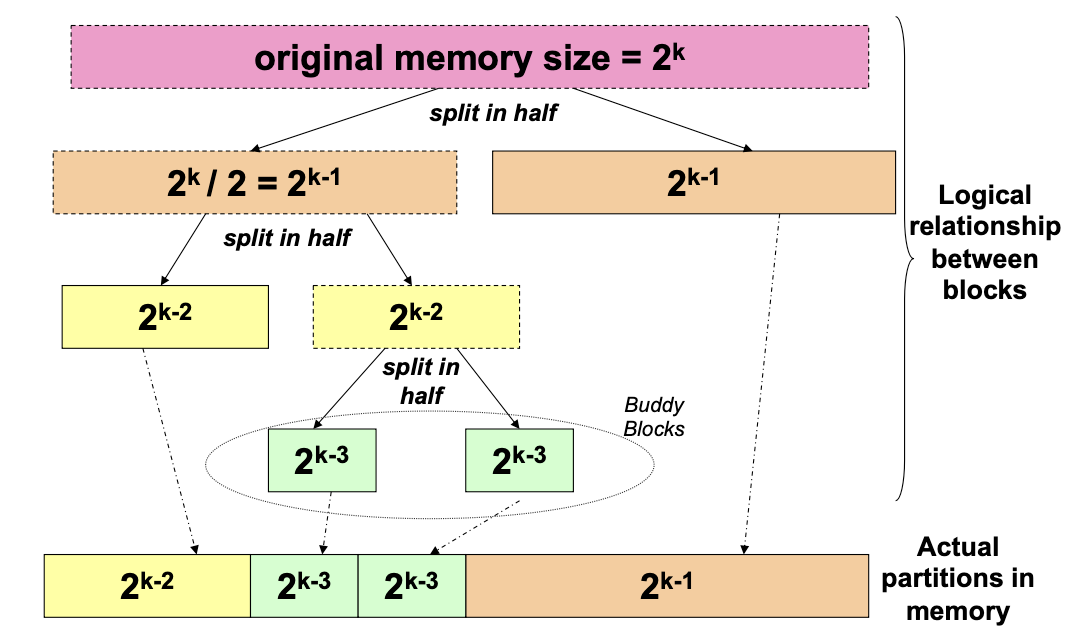
\includegraphics[width=0.9\linewidth]{14_buddy_system_overview.png}
        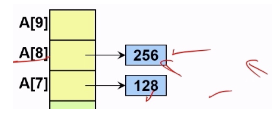
\includegraphics[width=0.7\linewidth]{15_buddy_system_linked_list.png}
        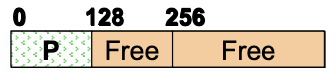
\includegraphics[width=0.6\linewidth]{16_buddy_system_layout.png}
        \item \underline{Allocation Algorithm:}
        \begin{enumerate}
          \item Find smallest S s.t. 2\textsuperscript{S} $\geq$ N 
          \item Check if \verb|A[S]| has free block
          \item Yes: Remove from list \& return
          \item No: Find smallest R from S+1 to K s.t. \verb|A[R]| has a free block $\rightarrow$ For R-1 to S, keep splitting until there is a block in S $\rightarrow$ Goto 2
        \end{enumerate}
        \item \underline{De-allocation Algorithm:}
        \begin{enumerate}
          \item To free a block B, check in \verb|A[S]| where 2\textsuperscript{S} == size of B
          \item If buddy C of B exists, remove B \& C from list, merge B \& C to get larger block B' $\rightarrow$ Goto step 1, where B $\leftarrow$ B'
          \item Else, insert B to list in \verb|A[S]| (buddy of B is not free yet)
        \end{enumerate}
        \item \underline{Locating Buddy:} B \& C are buddies of size 2\textsuperscript{S} if lowest S bits (0th - S-1th) of B \& C are identical \& Bit S is different
        \item \underline{Analysis of Buddy System:} (+): Best case O(1), worst case O(logn) allocation \& deallocation time (due to tree structure), (-): Has internal \& external fragmentation
      \end{itemize}
    \end{itemize}

    \section{Memory (Disjoint)}
    \textbf{ASSUMPTION REMOVED: Process fits in memory as contiguous piece $\rightarrow$ Process can now fit into memory but split into disjoint chunks}
    \subsection{Paging Scheme}
    \begin{itemize}
      \item \textbf{Overview:}
      \begin{itemize}
        \item \underline{Physical Frames:} Physical Memory is split into regions of fixed size (Frames are small VS partitions are big to accommodate largest process memory space)
        \item \underline{Logical Page:} Logical Memory of process is split into regions of same size
        \item Size of page == Size of frame (Pages of process are loaded into any available frame where logical memory is contiguous VS physical memory is disjoint)
      \end{itemize}
      \item \textbf{Page Table:}
      \begin{itemize}
        \item Maps Pages to Frames
        \item \underline{Address Translation}
        \begin{itemize}
          \item Method 1: PA = FrameNo. * sizeof(frame) + offset
          \item Method 2: PA = F * 2\textsuperscript{n} + O (given page/frame size of 2\textsuperscript{n} \& m bits of LA $\rightarrow$ P = most sig. m-n bits of LA, O = remaining n bits of LA $\rightarrow$ use P to find F via page table)
          \item Eg. Page size == 2\textsuperscript{2} bytes \& Page 00 maps to Frame 010, hence LA 00\underline{0}1 maps to 010\underline{01}, where 01 is offset
        \end{itemize}
      \end{itemize}
      \item \textbf{Fragmentation:} External fragmentation is not possible (every free frame can be used), Internal fragmentation is insignificant (logical memory space may not be multiple of page size $\rightarrow$ max 1 page per process not fully utilized)
      \item \textbf{Implementation of Paging Scheme:}
      \begin{itemize}
        \item OS stores Page Table info in PCB (Page Table is per process, not globally shared across processes)
        \item Memory context of process includes Page Table (or pointers to it since Page Tables are big)
        \item Requires 2 memory accesses for every memory reference (1st access to read PTE to get frame number, 2nd access to access actual memory item)
      \end{itemize}
      \item \textbf{Translation Look-Aside Buffer (TLB):} Aims to speed up address translation by acting as a cache for PTEs (TLB is a register in CPU, part of process' hardware context $\rightarrow$ page table is huge, cannot store entire page table within TLB, but TLB hit rate will still be high due to spatial \& temporal locality)
      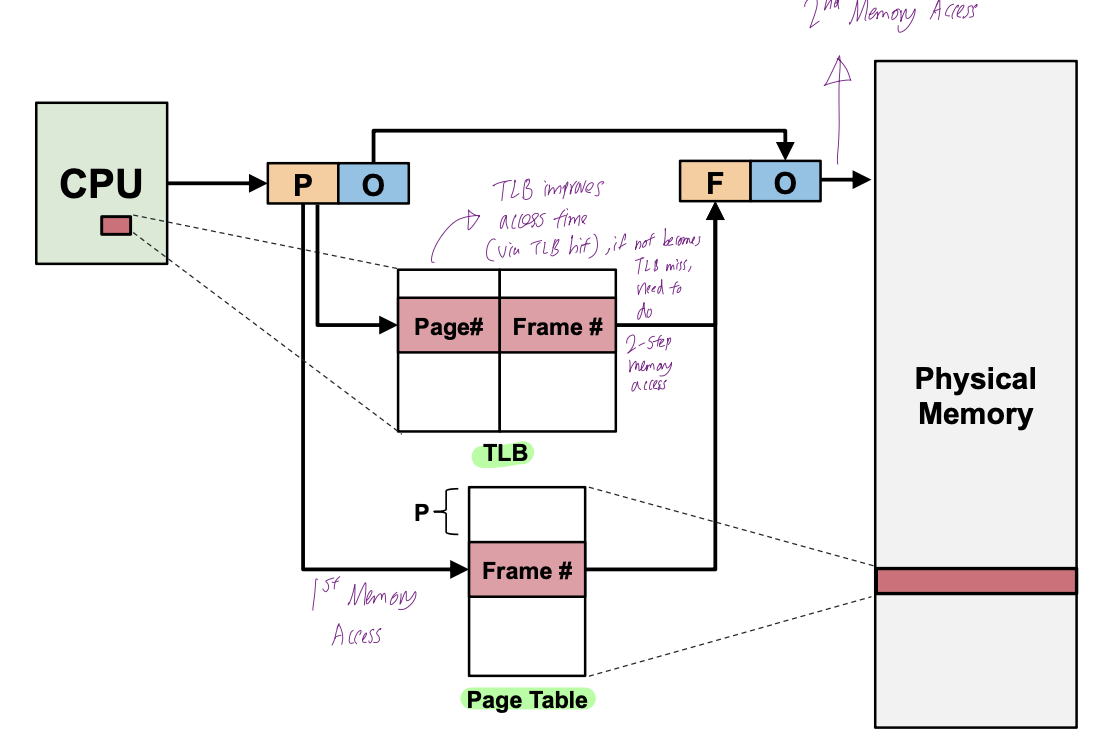
\includegraphics[width=0.8\linewidth]{17_TLB.png}
      \begin{itemize}
        \item \underline{Address Translation with TLB:} Use page number to search TLB $\rightarrow$ TLB-Hit (Frame no. retrieved, generate PA) OR TLB-Miss (Memory access to access page table, retrieve frame no. to generate PA \& update TLB)
        \item \underline{Avg. Memory Access Time (AMAT)} = P(TLB\textsubscript{hit}) * Latency(TLB\textsubscript{hit}) + P(TLB\textsubscript{miss}) * Latency(TLB\textsubscript{miss}) \\ Latency(TLB\textsubscript{hit}) = TLB Access + Actual Memory Access \\ Latency(TLB\textsubscript{miss}) = TLB Access + Page Table Access + Actual Memory Access
        \item \underline{Process Switching:} During context switching, Page Table \& TLB needs to be changed, but Frames remain same (TLB entries are flushed which causes many TLB misses to fill TLB when process resumes running)
      \end{itemize}
      \item \textbf{Protection Mechanism of Paging Scheme}
      \begin{enumerate}
        \item \underline{Access-right bit:} Each PTE has WRX bits (every memory access is checked against these bits in hardware; Child process has W = 0 initially for all pages after getting forked from parent which has W = 1 for some pages $\rightarrow$ W only changes to 1 for child when writing is needed)
        \item \underline{Valid bit:} Each PTE has Valid bit to indicate if page is valid to access by process (Some pages may be out of range for a process)
      \end{enumerate}
      \item \textbf{Page Sharing Mechanism of Paging Scheme:} Page table allows several processes to share same frame (\underline{Shared code page:} Common code like standard lib, syscalls; \underline{Copy-on-write}: Parent \& child share a frame until 1 process tries to change value in it)
    \end{itemize}

    \subsection{Segmentation Scheme}
    \begin{itemize}
      \item \textbf{Overview:}
      \begin{itemize}
        \item Logical memory space of a process == Collection of memory segments mapped into contiguous physical partitions of same size
        \item Each memory segment has (1): Name, (2): Limit; All memory reference == SegmentName + offset
      \end{itemize}
      \item \textbf{Segment Table:}
      \begin{itemize}
        \item Contains 2 fields per entry: Base \& Limit
        \item Each segment is mapped to a contiguous physical memory region with a base address \& limit
        \item Segment Table is much smaller than Page Table (only a few segments, i.e. Data, Code, Stack, Heap)
        \item \underline{Address Translation}: Given LA = \{SegID, Offset\}, SegID used to look up \{Base, Limit\} of segment in Segment Table $\rightarrow$ PA = Base + Offset (offset must be less than limit for valid access, or else seg fault error thrown)
      \end{itemize}
      \item \textbf{Pros:} Each segment is independent contiguous memory space, segments can grow/shrink (by updating segment limit), be protected/shared independently
      \item \textbf{Cons:} External Fragmentation (variable size contiguous memory regions)
    \end{itemize}

    \subsection{Segmentation with Paging Scheme}
    \begin{itemize}
      \item Each segment is composed of several pages instead of a contiguous memory region $\rightarrow$ Each segment has a Page table
      \item Segment can grow by allocating new page to add to its Page Table
      \item Segment Table's Base field is now base address of segment's Page Table instead of an address in physical memory
      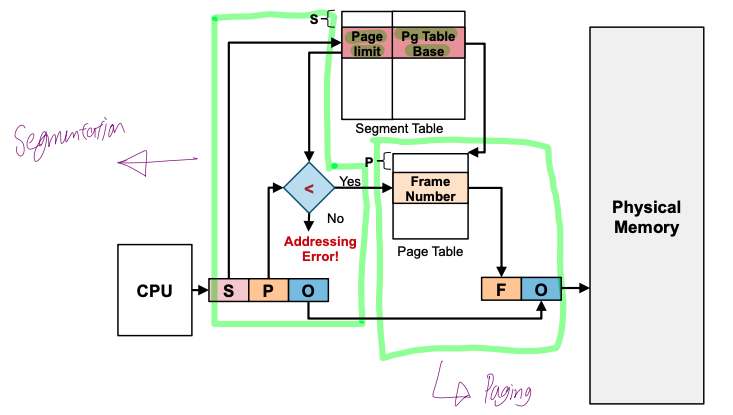
\includegraphics[width= 0.9\linewidth]{18_seg_with_pg.png}
    \end{itemize}

    \section{Memory (Virtual)}
    \textbf{ASSUMPTION REMOVED: Physical memory is large enough to contain $\geq$ 1 process with complete memory space}
    \subsection{Introduction}
    \begin{itemize}
      \item \textbf{Overview:}
      \begin{itemize}
        \item If Logical memory space of process \textgreater Physical memory, split logical address space into small chunks (Some chunks reside in physical memory, some stored in secondary storage)
        \item Page Table is still used for Logical to Physical address translation (with addition of \underline{Resident Bit} in PTE: Indicating whether page is resident in memory)
      \end{itemize}
      \item \textbf{Page Fault:} Occurs when CPU tries to access non-memory resident page $\rightarrow$ OS needs to bring non-memory resident page into physical memory (locate page in secondary storage, copy page into physical memory, update page table)
      \item \textbf{Benefits of Virtual Memory:} (1): Physical memory size no longer restrict size of logical memory address, (2): Page not needed can be on secondary storage, allowing efficient use of physical memory, (3): More processes can reside in memory ($\downarrow$ frames per process in physical memory)
      \item \textbf{Problems with Virtual Memory:}
      \begin{enumerate}
        \item \underline{Thrashing}: If memory access results in page fault most of the time, entire system slows down a lot ($\because$ secondary storage access time \textgreater physical memory access time) \textit{Cost of loading page is amortised by temporal \& spatial localities}
        \item \underline{Large no. of pages to allocate:} Large startup cost when a new large process is launched \textit{Solved by Demand Paging}
        \item \underline{Large Page Table:} No. of pages can be very big \textit{Solved by 2-level paging}
        \item \underline{Lack of frames to accommodate process:} No. of pages can be very big, far exceed no. of frames in physical memory $\rightarrow$ need to decide which page to replace \textit{Solved by Page Replacement Algos}
        \item \underline{No. of frames to allocate to a process:} Limited no. of physical memory frames $\rightarrow$ need to decide how to distribute frames amongst processes \textit{Solved by Frame Allocation Policies}
      \end{enumerate}
    \end{itemize}

    \subsection{Demand Paging}
    \begin{itemize}
      \item Aims to solve problem of large startup cost (Large no. of pages to allocate when new process is launched), reduce no. of frames per process
      \item \textbf{Mechanism:} Process starts with no memory resident page $\rightarrow$ Only allocate a page when there is a page fault
      \item \textbf{Pros:} Fast startup time for new process, small memory footprint
      \item \textbf{Cons:} Process may appear sluggish at start due to multiple page faults, which may lead to thrashing
    \end{itemize}

    \subsection{Page Table Structure}
    \begin{itemize}
      \item \textbf{Overview:} Virtual memory results in huge logical memory space, huge no. of pages, huge page table $\rightarrow$ Results in (1): \underline{High overhead} (Every process has huge page table \& page table is per process), (2): \underline{Page Table spanning several frames} (less ideal as frames are scattered throughout physical memory space)
      \item \textbf{Direct Paging:} Keeps all entries in single table
      \begin{itemize}
        \item e.g. Page size == 4KB, Virtual Addr is 64 bits long, Physical memory size == 16GB $\rightarrow$ No. of virtual pages = 2\textsuperscript{64}/2\textsuperscript{12} = 2\textsuperscript{52}, No. of physical pages = 2\textsuperscript{34}/2\textsuperscript{12} = 2\textsuperscript{22} (A lot less frames than pages)
        \item Given PTE size == 8B, Page table size = 2\textsuperscript{52}*8 = 2\textsuperscript{55}B per process (way higher than physical memory size, not paging method is not feasible)
      \end{itemize}
      \item \textbf{2-level Paging:} Aims to solve problem of Direct Paging by paging the page table (process may not use entire virtual memory space, full page table is wasteful)
      \begin{itemize}
        \item \underline{Mechanism:} VA is split into \{Bits (M) for page directory \#, Bits (P-M) for page \#, Bits for offset\#\} $\rightarrow$ Split Page Table into Page Tablets $\rightarrow$ If original Page Table has 2\textsuperscript{P} entries \& there are 2\textsuperscript{M} Page Tablets, each Page Tablet contains 2\textsuperscript{P-M} entries $\rightarrow$ Single Page Directory keeps track of Page Tablets
        \item \underline{Pros:} (1): Less overhead (\textit{Total overhead of page dir. + multiple page tablets \textless total overhead of single large page table}), (2): Enables page table structures to grow beyond size of a frame (\textit{Page dir. can point to page tablets residing in different disjoint frames}), (3): Can have empty entries in page dir. (\textit{Corr. page tablets do not need to be allocated})
        \item \underline{Cons:} 2 memory accesses needed to get frame no. (1st access for page dir., 2nd access for page tablet) $\rightarrow$ TLB can eliminate page table accesses, but TLB misses will need to traverse more page tables
      \end{itemize}
      \item \textbf{Hierarchical Page Table:} Radix tree structure, a table in each level of hierarchy is sized to fit in 1 frame, an invalid entry in any level means entire subtree does not exist
    \end{itemize}

    \subsection{Inverted Page Table}
    \begin{itemize}
      \item \textbf{Mechanism:} Keeps mapping of Frame \# to \{pid, Page \#\}, where pid == Process ID \& Page \# == Logical page no. in corr. process $\rightarrow$ page \# is not unique amongst processes, pid + page \# can uniquely identify a memory page $\rightarrow$ Entries are ordered by frame \#, to look up Page X, need to search whole table
      \item \textbf{Pros:} 1 table for all processes, huge savings
      \item \textbf{Cons:} Slow translation
      \item In practice, Inverted Page Table is used as auxiliary structure (find out which processes \& pages share frame X)
    \end{itemize}

    \subsection{Page Replacement Algorithms}
    \begin{itemize}
      \item \textbf{Overview:} No free frame during page fault $\rightarrow$ need to evict a memory page (Clean Page: not modified, no need write back to storage; Dirty page: modified, need to write back to storage)
      \item Good Page Replacement Algo should minimize total no. of page faults
    \end{itemize}
    \begin{enumerate}
      \item \textbf{Optimal Page Replacement (OPT)}
      \begin{itemize}
        \item Replace page that will not be needed again for longest period of time (Kick out MAX next use time)
        \item Guarantees min. no. of page faults
        \item \underline{Problems:} Not realizable as future knowledge of memory references is needed
      \end{itemize}
      \item \textbf{FIFO Page Replacement}
      \begin{itemize}
        \item Replace page that has the oldest loading time (Kick out MIN loaded at time)
        \item OS maintains queue of resident page numbers (1st page number gets kicked)
        \item \underline{Problems:} \# of frames $\uparrow$ $\rightarrow$ \# of page faults $\uparrow$ (Belady's Anomaly) as FIFO does not exploit temporal locality, bad performance in practice
      \end{itemize}
      \item \textbf{Least Recently Used (LRU)}
      \begin{itemize}
        \item Exploits temporal locality $\rightarrow$ Replace page that has not been used in longest time (Kick out MIN last use time)
        \item Aims to approx. OPT \& does not suffer from Belady's Anomaly
        \item Need to keep track of "Last Use Time"
          \begin{itemize}
            \item \underline{Counter:} Time counter that is incremented for every memory reference (Each PTE has a Last Use Time field), but need to search through all pages to find min. last use time, and overflow might occur as time-of-use keeps $\uparrow$
            \item \underline{Stack:} Maintain a stack of page no., if page X is referenced, remove X from stack \& push X on top of stack, replace page at bottom of stack (no need search all entries), but this is not pure stack, hard to implement
          \end{itemize}
      \end{itemize}
      \item \textbf{Second Chance (CLOCK)}
      \begin{itemize}
        \item Modified FIFO give 2nd chance to pages that were accessed
        \item Each PTE has a Reference Bit (1: Accessed since last reset, 0: Not accessed)
        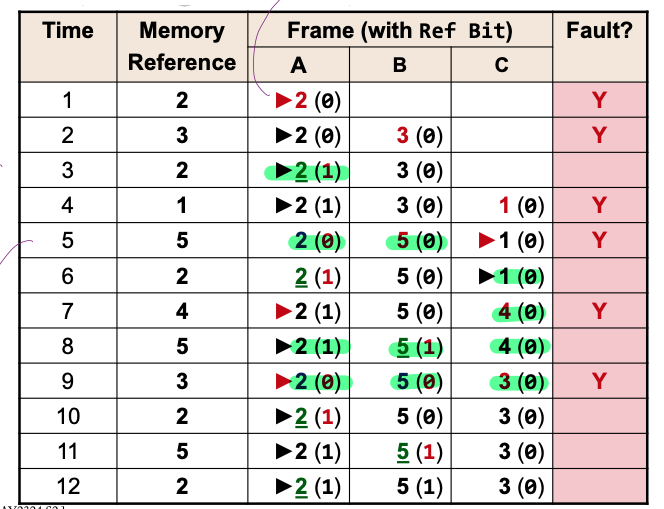
\includegraphics[width=0.9\linewidth]{19_second_chance_algo.png}
        \item \underline{Algorithm:} \\
        1. Oldest FIFO page is selected (Victim Page)\\
        2. If Ref Bit == 0, page is replaced\\
        3. If Ref Bit  == 1, page is skipped, Ref Bit reset to 0, next FIFO page is selected, goto (2)
        \item Degenerates into FIFO when Ref Bits of all pages == 1
        \item \underbar{Implementation:} Circular list of all pages, pointer pointing to next potential victim page, finding a victim (advance until 1st page with '0' bit, clear any bits as pointer passes through)
      \end{itemize}
    \end{enumerate}

    \subsection{Frame Allocation Policies}
    \begin{itemize}
      \item \textbf{Overview:} Consider N frames \& M processes competing for frames
      \begin{enumerate}
        \item \underline{Equal Allocation:} Each process gets N/M frames
        \item \underline{Proportional Allocation:} Each process gets size\textsubscript{p}/size\textsubscript{total} * N frames
      \end{enumerate}
      \item \textbf{Local VS Global Replacement}
      \begin{enumerate}
        \item \underline{Local Replacement:} Victim page is selected among pages of a process that causes page fault, thrashing is limited to 1 process (\textit{Pros: \# of frames allocated to process remains constant, stable performance btw. runs, Cons: Frames allocated may be insufficient})
        \item \underline{Global Replacement:} Victim page is selected among all frames (Process P can take frame from Process Q by evicting Q's frame) (\textit{Pros: Process that needs more frames can get from those that need less, Cons: Badly behaved process can steal frames from other process, can cause other process to thrash too})
      \end{enumerate}
      \item \textbf{Working Set:} Set of pages referenced by a process that is relatively constant in a period of time, occurs in stable region of Working Set Model
      \begin{itemize}
        \item When function is executing, references are constant VS When function terminates, references change to another set
        \item Aims to find right \# of frames for a process
      \end{itemize}
    \end{itemize}
    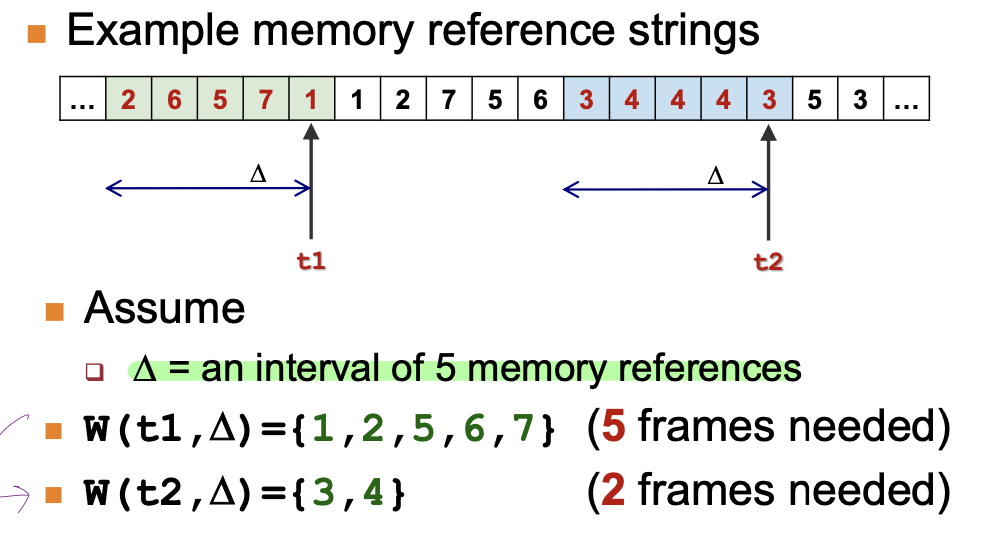
\includegraphics[width=0.8\linewidth]{20_working_set.png}

    \section{File Systems Introduction}
    \subsection{File System}
    \begin{itemize}
      \item File system provides abstraction on top of physical media, high level resource management, protection btw. processes \& users, sharing btw. processes \& users
      \item \textbf{Memory VS File Management} \\
        \underline{Underlying Storage:} RAM $\vert$ Disk \\
        \underline{Access Speed:} Constant $\vert$ Variable disk I/O time \\
        \underline{Unit of Addressing:} Physical memory addressing $\vert$ Disk sector \\
        \underline{Usage:} Address space for process, implicit when process runs $\vert$ Non-volatile data, explicit access \\
        \underline{Organisation:} Paging/Segmentation $\vert$ ext(Linux), FAT (Windows), HFS(MacOS)
    \end{itemize}

    \subsection{File}
    \begin{itemize}
      \item \textbf{Basic Description:} File represents a logical unit of info created by process, contains Data \& Metadata
      \item \textbf{File Metadata:} \underline{File Name} (Human readable reference to file), \underline{Identifier} (Unique ID for file used internally by FS), \underline{Type} (Indicate different types of files such as ASCII, Binary files, directories $\vert$ file types can be distinguished via file extension or magic number stored at file beginning), \underline{Size} (current sizer of file in bytes, words or blocks), \underline{Protection} (RWX permission bits for Owner, Group, Universe OR Access Control List), \underline{Time,} \underline{ date, owner info, Info for FS to determine how to access file}
      \item \textbf{File Data:}
      \begin{itemize}
        \item \underline{Structure:} (1): \underline{Array of bytes} \textit{(Each byte has unique offset from file start)}, (2): \underline{Fixed Length Record} \textit{(Array of records, can jump to any record easily, where Offset of Nth record == Sizeof Record *(N-1))}, (3): \underline{Variable Length Record} \textit{(Flexible but harder to locate a record)}
        \item \underline{Access Methods:} (1): \underline{Sequential Access} \textit{(Data is read in order from beginning, cannot skip but can be rewound)}, (2): \underline{Random Access} \textit{(Data can be read in any order in bytes)}, (3): \underline{Direct Access} \textit{(Random access to any records directly, used for fixed length records, useful for large \# of records}
        \item \underline{Generic Operations:} Create, Open, Read, Write, Repositioning \textit{(move current position to new location)}, Truncate \textit{(Removes data btw. specified position to EOF)}
      \end{itemize}
      \item \textbf{System Calls:}
      \begin{enumerate}
        \item \verb|int open(char *path, int flags)|
        \item \verb|int read(int fd, void *buf, int n)|
        \item \verb|int write(int fd, void *buf, int n)|
        \item \verb|off_t lseek(int fd, off_t offset, int whence)| (Offset(+) $\rightarrow$ move forward, Offset(-) $\rightarrow$ move backward $\vert$ Whence: point of reference for interpreting offset, SEEKSET: absolute offset from start, SEEKCUR: relative offset from current position, SEEKEND: relative offset from end of file)
        \item \verb|int close(int fd)| (fd is no longer used \& kernel can remove associated data structures, fd can be reused later $\vert$ Process termination automatically closes all open files)
      \end{enumerate}
      NOTE: Default File Descriptors: STDIN(0), STDOUT(1), STDERR(2)
    \end{itemize}

    \subsection{File Information}
    \begin{itemize}
      \item \textbf{Info for Opened Files:} (1): \underline{File Pointer} (Keep track of current position within file), (2): \underline{File Descriptor} (Unique ID of file), (3): \underline{Disk Location} (Actual file location on disk), (4): \underline{Open Count} (Tracks \# of processes which has file opened)
      \item \textbf{Tables tracking file information (All in Kernel Space):}
      \begin{enumerate}
        \item \underline{Per Process Open File Table}: Found in PCB, keeps track of open files for 1 process, each entry points to SWOFT entry
        \item \underline{System wide Open File Table}: Keeps track of all open files in system, each entry points to a V-node entry
        \item \underline{System wide V-node Table}: Links with file on physical drive, contains info about file's physical location
      \end{enumerate}
      \item Process makes file syscalls with file descriptor
      \item Every time a new file is opened by a process, a new FD entry is added to process' PPOFT
      \item A file can be opened twice by 2 processes $\rightarrow$ Need to have different entries for same file in SWOFT with different file offset (P0 may read/write to different portion of file from P1)
      \item Parent \& Child processes use same SWOFT entry (only 1 offset needed)
      \item Open Count == 0 $\rightarrow$ delete entry from table
      \item \underline{I-node:} File data structure that stores info about file 
    \end{itemize}

    \subsection{Directory}
    \begin{itemize}
      \item Provides logical grouping of files, keeps track of files
      \item \textbf{Single Level:} Only can support unique names
      \item \textbf{Tree Structure:} Can have same file names as long as files are in different directories
      \item \textbf{Directed Acyclic Graph:}
      \begin{itemize}
        \item A file can be shared (only 1 copy of actual content but appears in multiple directories, 2 file names referring to same file content)
        \item Facilitated by Unix's Hard Link (Dir A is owner of File F, Dir B wants to share F $\rightarrow$ A \& B have separate pointers to F in disk)
        \item Low overhead (Only pointers are added in directory), Deletion problems can be settled by Open Count (Delete file when 0)
      \end{itemize}
      \item \textbf{General Graph:}
      \begin{itemize}
        \item Cycles are allowed (Hard to traverse since need to prevent infinite looping, hard to determine when to remove file/dir)
        \item Facilitated by Unix's Symbolic Link (special link file that contains path name of file)
        \item If Symbolic Link is deleted $\rightarrow$ Link file is deleted, but not file $\vert$ If file is deleted $\rightarrow$ File is deleted, but Link File remains as dangling link
        \item High overhead (Link File requires a separate I-node \& takes up disk space)
      \end{itemize}
    \end{itemize}

    \section{File Systems Implementation}
    \subsection{Overview}
    \begin{itemize}
      \item \textbf{General Disk Structure:} 1D array of logical blocks (Logical Block: Small accessible unit, mapped into disk sectors) $\vert$ 1 Directory is allocated a logical block $\vert$ 1 file is split \& allocated a few logical blocks
      \item \textbf{General Disk Organisation:}
      \begin{enumerate}
        \item \underline{Master Boot Record}: Located at sector 0  with Partition Table \& Simple Boot Code (Activates partitions by checking if they have bootable device)
        \item \underline{Partition:} Each partition contains an independent file system (eg. Windows in partition C:, Linux in partition D:)
        \item \underline{OS Boot Block:} Code to load OS into RAM
        \item \underline{Partition Details:} Total \# of blocks, \# \& location of free/allocated blocks
        \item \underline{Directory Structure:} Tracks files in a directory, map file name to file info
        \item \underline{Files Info:} File Metadata
        \item \underline{File Data:} File content
      \end{enumerate}
      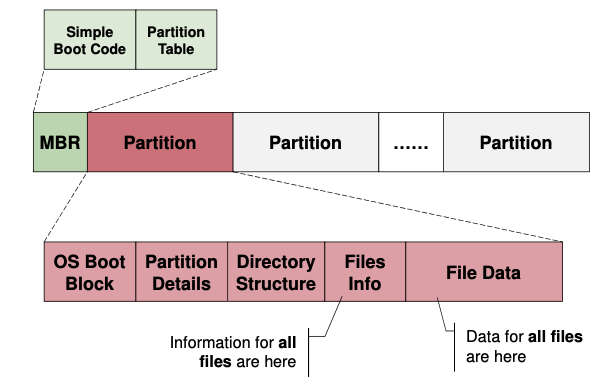
\includegraphics[width=1.0\linewidth]{21_disk_organisation.png}
    \end{itemize}

    \subsection{Implementing File (File Info + File Data)}
    \textbf{Overview:} A file is a collection of logical blocks $\rightarrow$ Need to allocate file data to logical blocks via allocation schemes (Internal Fragmentation occurs when file size != multiple of logical blocks)
    \begin{enumerate}
      \item \textbf{Contiguous Allocation}
      \begin{itemize}
        \item Allocates consecutive disk blocks to a file $\vert$ exists a table in Files Info to keep track of \{file name, start block \#, length in terms of blocks\} entries
        \item \underline{Pros:} Simple to track, fast access (Contiguous logical blocks are closely located on same/adjacent disk sectors, no need to move disk head a lot)
        \item \underline{Cons:} External Fragmentation (Holes created btw. logical blocks occupied by files), File size must be specified before (fit file in a appro. range of contiguous logical blocks)
      \end{itemize}
      \item \textbf{Linked List Allocation}
      \begin{itemize}
        \item Linked list of disk blocks (Each disk block stores next disk block \# via pointer \& actual file data) $\vert$ Last block in linked list has special value $\vert$ exists a table in File Info to keep track of \{File Name, Start Block \#, End Block \# \} entries (End block makes appending operation faster coz no need traverse linked list)
        \item \underline{Pros:} Solves Fragmentation problem (Logical blocks need not be contiguous)
        \item \underline{Cons:} Random access in file is slow (blocks can be in different disk sectors), Additional overhead to store pointers (part of disk block used for pointer), Less reliable (pointers may be wrong)
      \end{itemize}
      \item \textbf{Linked List V2.0 FAT Allocation}
      \begin{itemize}
        \item Move all block pointers into File Allocation Table (FAT) which is in memory 
        \item Exists a table to track \{File Name, Start Block \#\} (No need store End Block \# since FAT is more efficient) $\vert$ FAT entry is of form \{Current Block \#, (FREE, Next Block \#, EOF or BAD)\}
        \item \underline{FAT Version:} FAT16 (2\textsuperscript{16} entries, entry size == 16 bits since address of each FAT entry is stored) $\vert$ FAT32 (2\textsuperscript{32}, entry size == 32 bits)
        \item \underline{Pros:} Faster random access (Linked list traversal is in memory instead of hard disk)
        \item \underline{Cons:} Consume lots of memory (FAT tracks all disk blocks in partition)
      \end{itemize}
      \item \textbf{Indexed Allocation}
      \begin{itemize}
        \item Each file has an index block (contains an array of disk block addresses, IndexBlock[N] == Nth block address, Each address is pointer to actual logical block)
        \item \underline{Pros:} Less memory overhead (only Index Block needs to be in memory), Fast direct access (Directly access via array indexing, no linked list traversals)
        \item \underline{Cons:} Limited max file size (max \# of blocks == \# of Index Block entries), Index Block overhead (block is used for Index Block instead of data storage)
      \end{itemize}
      \item \textbf{Indexed Allocation Variants}
      \begin{itemize}
        \item Allow for larger files (via multiple index blocks)
        \item \underline{Linked List Scheme:} Keep linked list of Index Blocks (but expensive due to traversal cost)
        \item \underline{Multi-level Index:} Similar idea to multi-level paging
        \item \underline{Combined Scheme:} Use Direct Index (fast access to small files), Multi-level index (large files)
        \item \underline{Eg. of Combined Scheme: UNIX I-Node}
        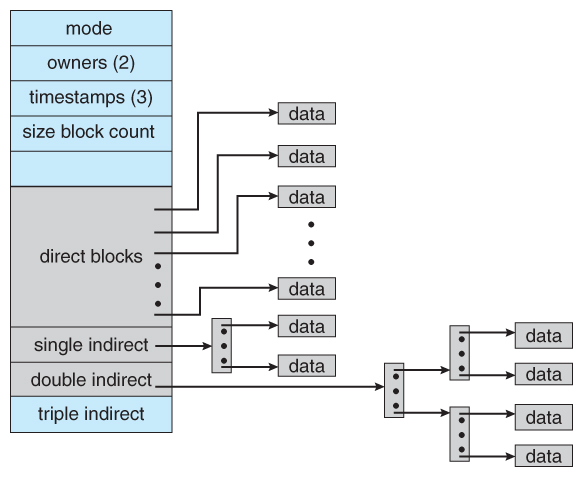
\includegraphics[width=0.8\linewidth]{22_unix_inode.jpeg}
        \begin{itemize}
          \item Every file/dir has a I-node data block associated to it (I-node consists of direct, indirect blocks)
        \end{itemize}
      \end{itemize}
    \end{enumerate}

    \subsection{Free Space Management (Partition Details)}
    \begin{itemize}
      \item \textbf{Overview:} Need to know which disk block is free to perform file allocation (Partition Details maintain free space information, remove free disk block from free space list for allocate, add free disk block to free space list for free)
      \item \textbf{Bitmap:} Each disk block is represented by 1 bit (Bit 0: occupied block, Bit : free block $\vert$ provides good set of manipulation but need to keep in memory for efficiency reason)
      \item \textbf{Linked List:} Linked list of disk blocks (Each disk block contains a \# of few disk block numbers OR a pointer to next free space disk block $\vert$ Easy to locate free block, only 1st pointer needs to be in memory, but high overhead)
    \end{itemize}

    \subsection{Implementing Directory (Directory Structure)}
    \begin{itemize}
      \item \textbf{Overview:} Keeps track of files in directory \& maps file name to file info $\vert$ Sub-directory stored as file entry with special type in a directory
      \item \textbf{Linear List}: Directory consists of a linear list where each entry represents a file (stores file name \& metadata \& file info OR pointer to file info) $\rightarrow$ but requires linear search (inefficient for large directories)
      \item \textbf{Hash Table:} Directory contains a hash table of size N where File Name is hashed into index K where 0 $\leq$ K $\leq$ N-1 (Fast lookup, but may have collisions)
      \item \textbf{File Information:} (1): Store all file info in a directory entry, (2): Store only file name \& points to some data structure for other information
      \item \textbf{FAT16 Directory Entry:}
      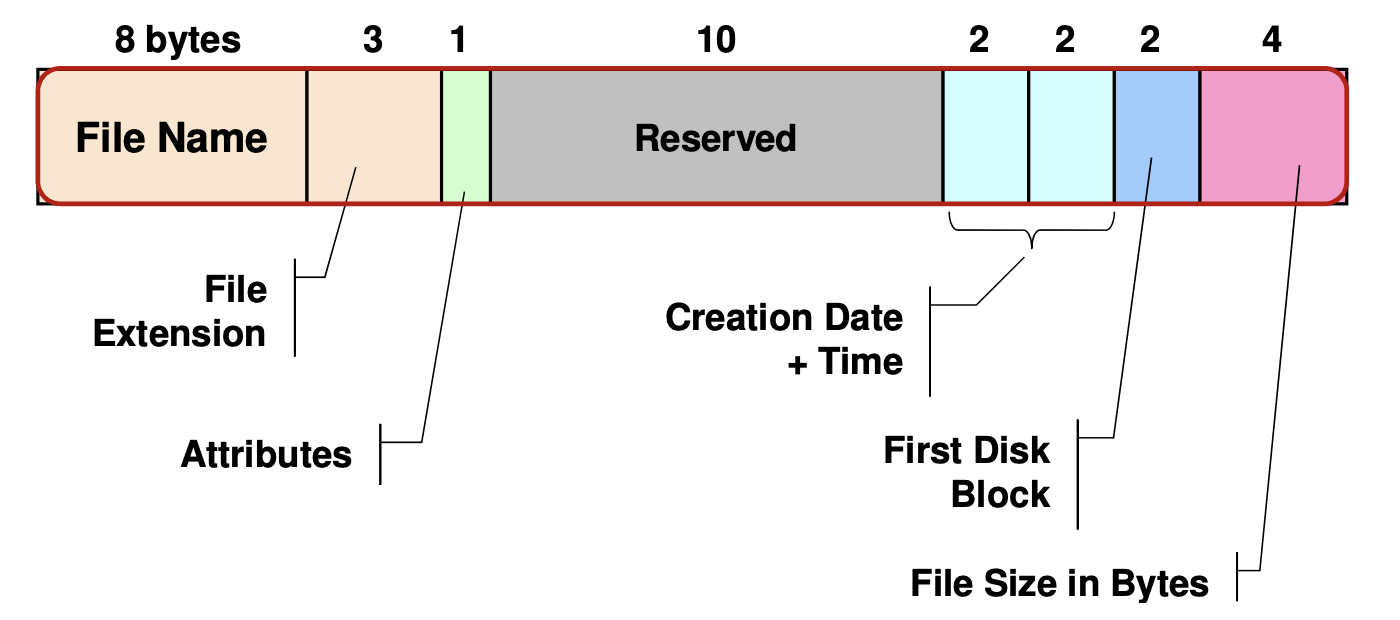
\includegraphics[width=1.0\linewidth]{23_fat16_dir_entry.png}
      \item \textbf{Ext2 Directory Entry:}
      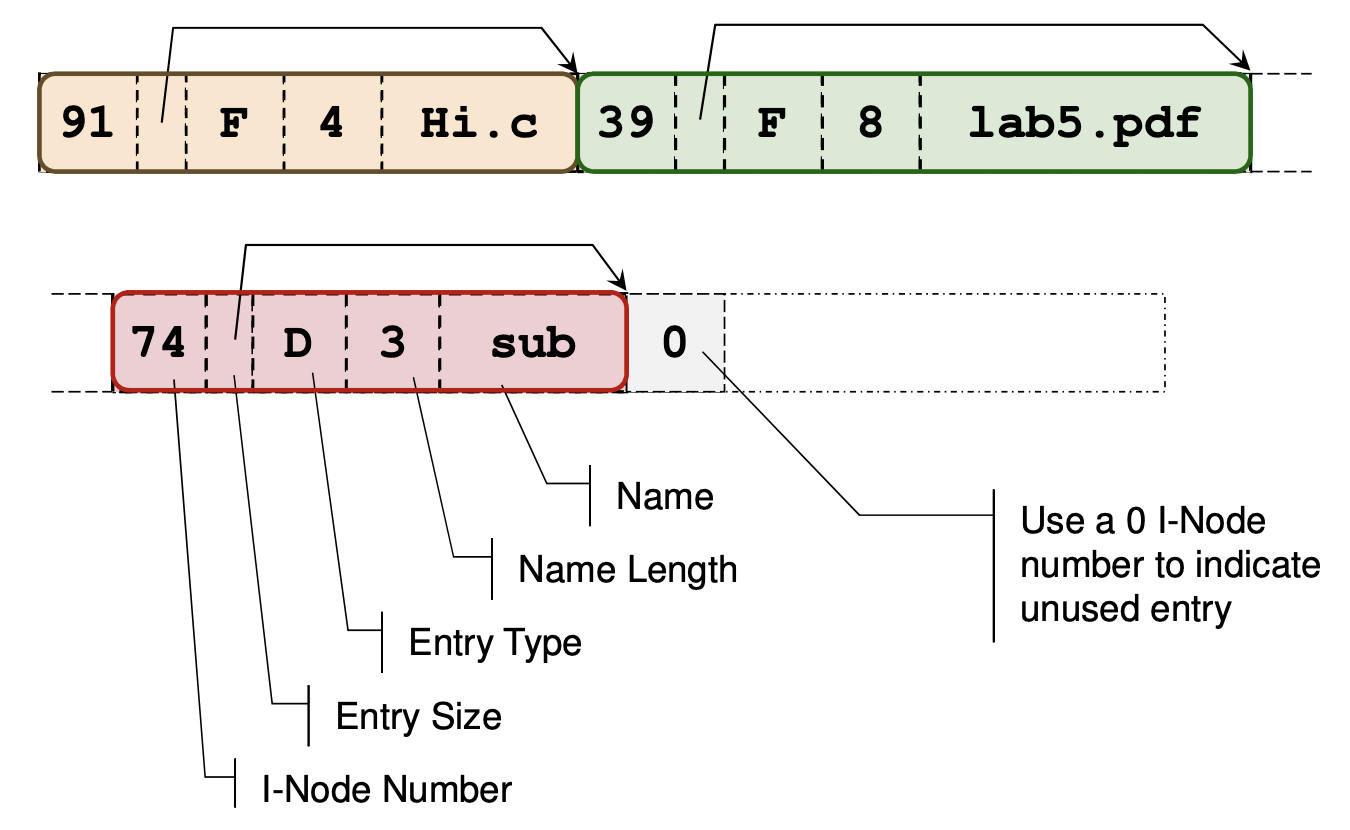
\includegraphics[width=1.0\linewidth]{24_ext2_dir_entry.png}
    \end{itemize}

    \subsection{File System in Action}
    \textbf{File Creation (Create File F):}
    \begin{enumerate}
      \item Use full path name to locate parent directory
      \item Search for file name F to avoid duplicates
      \item Use Free Space List to find free disk blocks
      \item Add an entry to parent directory (with relevant file info, file name, disk block info)
    \end{enumerate}
    \textbf{File Opening (Process P opens File F):}
    \begin{enumerate}
      \item Use full path name to locate File F
      \item When F is located, F's file info is loaded into new entry E in system-wide table \& V in I-node table if not already present
      \item Create an entry in P's table to point to E \& pointer from E's entry to V
      \item Return file descriptor for further read/write operation
    \end{enumerate}
  \end{multicols*}
\end{document}
